\item The unit vectors along the mutually perpendicular $x, y$ and $z$ axes are $\hat{i}, \hat{j}$ and $\hat{k}$ respectively. Consider the plane $z = 0$ and two vectors $\vec{a}$ and $\vec{b}$ on that plane such that $\vec{a} \neq \alpha \vec{b}$ for any scalar $\alpha$. A vector perpendicular to both $\vec{a}$ and $\vec{b}$ is \rule{1cm}{0.01pt}.
\hfill{(IN 2020)}
\begin{enumerate}
\begin{multicols}{4}
\item $\hat{k}$
\item $\hat{i} - \hat{j}$
\item $-\hat{j}$
\item $\hat{i}$
\end{multicols}
\end{enumerate}
\item A set of linear equations is given in the form $\vec{A}\vec{x} = \vec{b}$, where $\vec{A}$ is a $2 \times 4$ matrix with real number entries and $\vec{b} \neq 0$. Will it be possible to solve for $\vec{x}$ and obtain a unique solution by multiplying both left and right sides of the equation by $\vec{A}^{\top}$  and inverting the matrix $\vec{A}^{\top} \vec{A}$? Answer is \rule{1cm}{0.01pt}.
\hfill{(IN 2020)}
\begin{enumerate}
\item Yes, it is always possible to get a unique solution for any $2 \times 4$ matrix $\vec{A}$.
\item No, it is not possible to get a unique solution for any $2 \times 4$ matrix $\vec{A}$.
\item Yes, can obtain a unique solution provided the matrix $\vec{A}^{\top} \vec{A}$ is well conditioned
\item Yes, can obtain a unique solution provided the matrix $\vec{A}$ is well conditioned
\end{enumerate}
\item Consider the matrix 
\begin{align*}
\vec{M} = \myvec{1 & -1 & 0 \\ 1 & -2 & 1 \\ 0 & -1 & 1}.
\end{align*}
 One of the eigenvectors of $\vec{M}$ is
\hfill{(IN 2020)}
\begin{enumerate}
\begin{multicols}{4}
\item
\myvec{ -1 \\ 1 \\ 1 }
\item 
\myvec{ 1 \\ 1 \\ -1 }
\item
\myvec{ -1 \\ -1 \\ 1 }
\item
\myvec{ 1 \\ 1 \\ 1 }
\end{multicols}
\end{enumerate}
\item A straight line drawn on an x-y plane intercepts the $X$ axis at $-0.5$ and the $Y$ axis at $1$. The equation that describes this line is \rule{1cm}{0.01pt}.
\hfill{(IN 2020)}
\begin{enumerate}
\begin{multicols}{4}
\item $y = -0.5 x + 1$
\item $y = x - 0.5$
\item $y = 0.5x - 1$
\item $y = 2x + 1$
\end{multicols}
\end{enumerate}
\item $I_1, I_2$ and $I_3$ in the \figref{fig:q13} are mesh currents. The correct 
set of mesh equations for these currents, in matrix form, is \rule{1cm}{0.01pt}.
\hfill{(IN 2020)}
\begin{figure}[H]
\centering
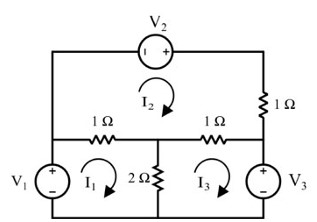
\includegraphics[width=0.5\columnwidth]{GATE/2020/IN/figs/q13.jpg}
\caption{}
\label{fig:q13}
\end{figure}
\begin{enumerate}
\begin{multicols}{2}
\item
\begin{align*}
\myvec{ 3 & -1 & -2 \\ -1 & 3 & -1 \\ -2 & -1 & 3 } \myvec{ I_1 \\ I_2 \\ I_3 } = \myvec{ V_1\\ V_2 \\ -V_3 }
\end{align*}
\item
\begin{align*}
\myvec{ 3 & -1 & -2 \\ -1 & 3 & -1 \\ -2 & -1 & -3 } \myvec{ I_1 \\ I_2 \\ I_3 } = \myvec{ V_1 \\ V_2 \\ V_3 }
\end{align*}
\item 
\begin{align*}
\myvec{ -3 & -1 & -2 \\ -1 & 3 & -1 \\ -2 & -1 & 3 } \myvec{ I_1 \\ I_2 \\ I_3 } = \myvec{ V_1 \\ V_2 \\ -V_3 }
\end{align*}
\item 
\begin{align*}
\myvec{ 1 & -1 & -2 \\ -1 & 2 & -1 \\ -2 & -1 & 3 } \myvec{ I_1 \\ I_2 \\ I_3 } = \myvec{ V_1 \\ V_2 \\ V_3 }
\end{align*}
\end{multicols}
\end{enumerate}


\item Consider the function $f\brak{x, y} = x^2 + y^2$. The minimum value the function attains on the line $x + y = 1$ \brak{\text{rounded off to one decimal place}} is \rule{1cm}{0.01pt}.
\hfill{(IN 2020)}
\item Consider the finite sequence $X = \brak{1, 1, 1}$. The Inverse Discrete Fourier Transform \brak{IDFT} of $X$ is given as $\brak{x\brak{0}, x\brak{1}, x\brak{2}}$. The value of $x\brak{2}$ is 
\hfill{(IN 2020)}

